\documentclass[]{standalone}

% More defined colors
\usepackage[dvipsnames]{xcolor}
\definecolor{gray_black}{RGB}{18,54,147}
\definecolor{royal_blue}{RGB}{0,83,214}


\usepackage{tikz}
\usetikzlibrary{positioning, shapes.geometric}

\tikzstyle{block} = [rectangle, rounded corners, minimum width=0.5cm, minimum height=0.5cm,
                    text centered, line width=0mm, inner sep=0.2cm, draw=royal_blue]  %, text width=3cm
\tikzstyle{arrow} = [thick,-latex, gray_black]

\tikzstyle{Func} = [rectangle, rounded corners, minimum width = 6mm, minimum height = 6mm, draw=blue!50, fill = blue!20, inner sep = 0cm]
\tikzstyle{Sum} = [circle, minimum width = 4mm, minimum height = 4mm, draw=black!50, fill = black!20, inner sep = 0cm, text = black]

\begin{document}
 
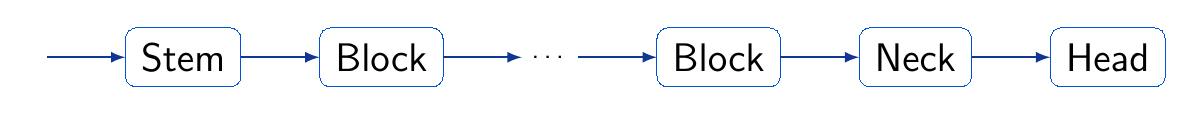
\begin{tikzpicture}

    \node[] (start) at (0,0) {};
    \node[block] (stem) [right= of start] {\sffamily \Large Stem};
    \node[block] (block1) [right= of stem] {\sffamily \Large Block};
    \node[] (dots) [right= of block1] {\sffamily \dots};
    \node[block] (block2) [right= of dots] {\sffamily \Large Block};
    \node[block] (neck) [right= of block2] {\sffamily \Large Neck};
    \node[block] (head) [right= of neck] {\sffamily \Large Head};

    \draw[arrow] (start) to (stem);
    \draw[arrow] (stem) to (block1);
    \draw[arrow] (block1) to (dots);
    \draw[arrow] (dots) to (block2);
    \draw[arrow] (block2) to (neck);
    \draw[arrow] (neck) to (head);

\end{tikzpicture}

\end{document}